\qnhead{Using SparQLed}

If no problem, the SparQLed (Figure~\ref{fig:sparqled}) webapp is available at:

\bigskip
\begin{raggedleft}
\framebox[\linewidth][l]{
    \texttt{
        \url{http://localhost:8080/sparqled/}
    }
}
\end{raggedleft}

\begin{marginfigure}
    \resizebox{\linewidth}{!}{
    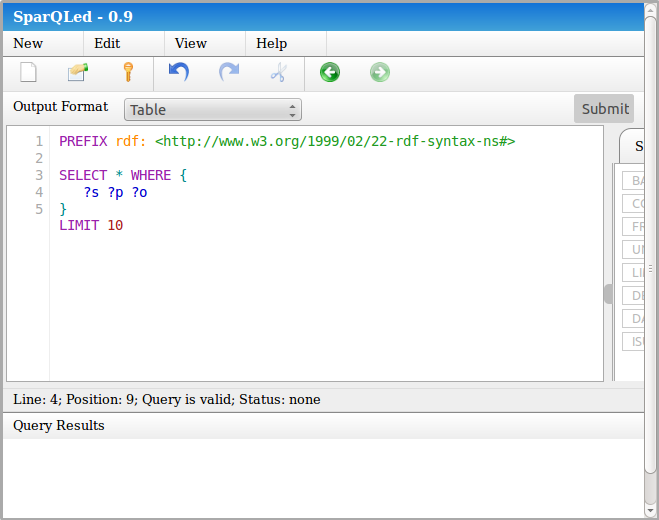
\includegraphics[scale=1]{figures/window.png}}
    \caption{The SparQLed editor}
    \label{fig:sparqled}
\end{marginfigure}
 
In case the webapp does not work properly, please have a look at the logs:

\bigskip
\begin{raggedleft}
\framebox[\linewidth][l]{
    \parbox[r]{\linewidth}{\texttt{
        \$ tail -f \$CATALINA\_BASE/logs/catalina.out\\\hspace{0.002cm}
        \$ tail -f /path/to/sindice/home/log/sparqled/sparqled.log
    }}
}
\end{raggedleft}

The SparQLed\footnote{\textcolor{blue}{A live version and a screencast are available at \url{http://hcls.sindicetech.com/sparql-editor/}}} editor gives you four types of recommendations, i.e., class, predicate, relationship between variables and named graphs.

In order to get recommendations you have to hit \texttt{Ctrl + Space} at the desired position in the query. The recommendations generated by the editor will be provided in the form of a drop down list. The user can then select one entry from the drop down box that matches his criteria. Keyword (resp., prefix) search is also possible by typing a word (resp., prefix), followed by \texttt{Ctrl + Space}.

